\subsection{Failures in PIR Sensors -- A Taxonomy} 
\label{subsec:taxonomy} 

%%%%%%%%%%%%%%%%
% FAILURE PHOTOGRAPHS
%%%%%%%%%%%%%%%%
\begin{figure}%[t]
	\centering
	\small
	\begin{subfigure}[t]{0.24\textwidth}
		\centering
		\includegraphics[width=\textwidth]{figures/platform/failure_photographs/WorkingSensor-proper.jpg}
		\caption{\footnotesize Working Sensor}
		\label{fig:working}
	\end{subfigure}
	\hspace{0.10ex}%
	\begin{subfigure}[t]{0.24\textwidth}
		\centering
		\includegraphics[width=\textwidth]{figures/platform/failure_photographs/ClassI-LensCapRemoved-annotated-jpg.jpg}
		\caption{Lens Cap Fallen Off}
		\label{fig:failure_photo1}
	\end{subfigure}
	\hspace{0.10ex}
	\begin{subfigure}[t]{0.24\textwidth}
		\centering
		\includegraphics[width=\textwidth]{figures/platform/failure_photographs/ClassI-LensCapDislogdged-annotated-jpg.jpg}
		\caption{\footnotesize Lens Cap Dislocated}
		\label{fig:failure_photo2}
	\end{subfigure}	
	\hspace{0.10ex}
	\begin{subfigure}[t]{0.24\textwidth}
		\centering
		\includegraphics[width=\textwidth]{figures/platform/failure_photographs/ClassII-LensCapDeformed-annotated-jpg.jpg}
		\caption{Lens Cap Deformed}
		\label{fig:failure_photo3}
	\end{subfigure}
	\begin{subfigure}[t]{0.24\textwidth}
		\centering
		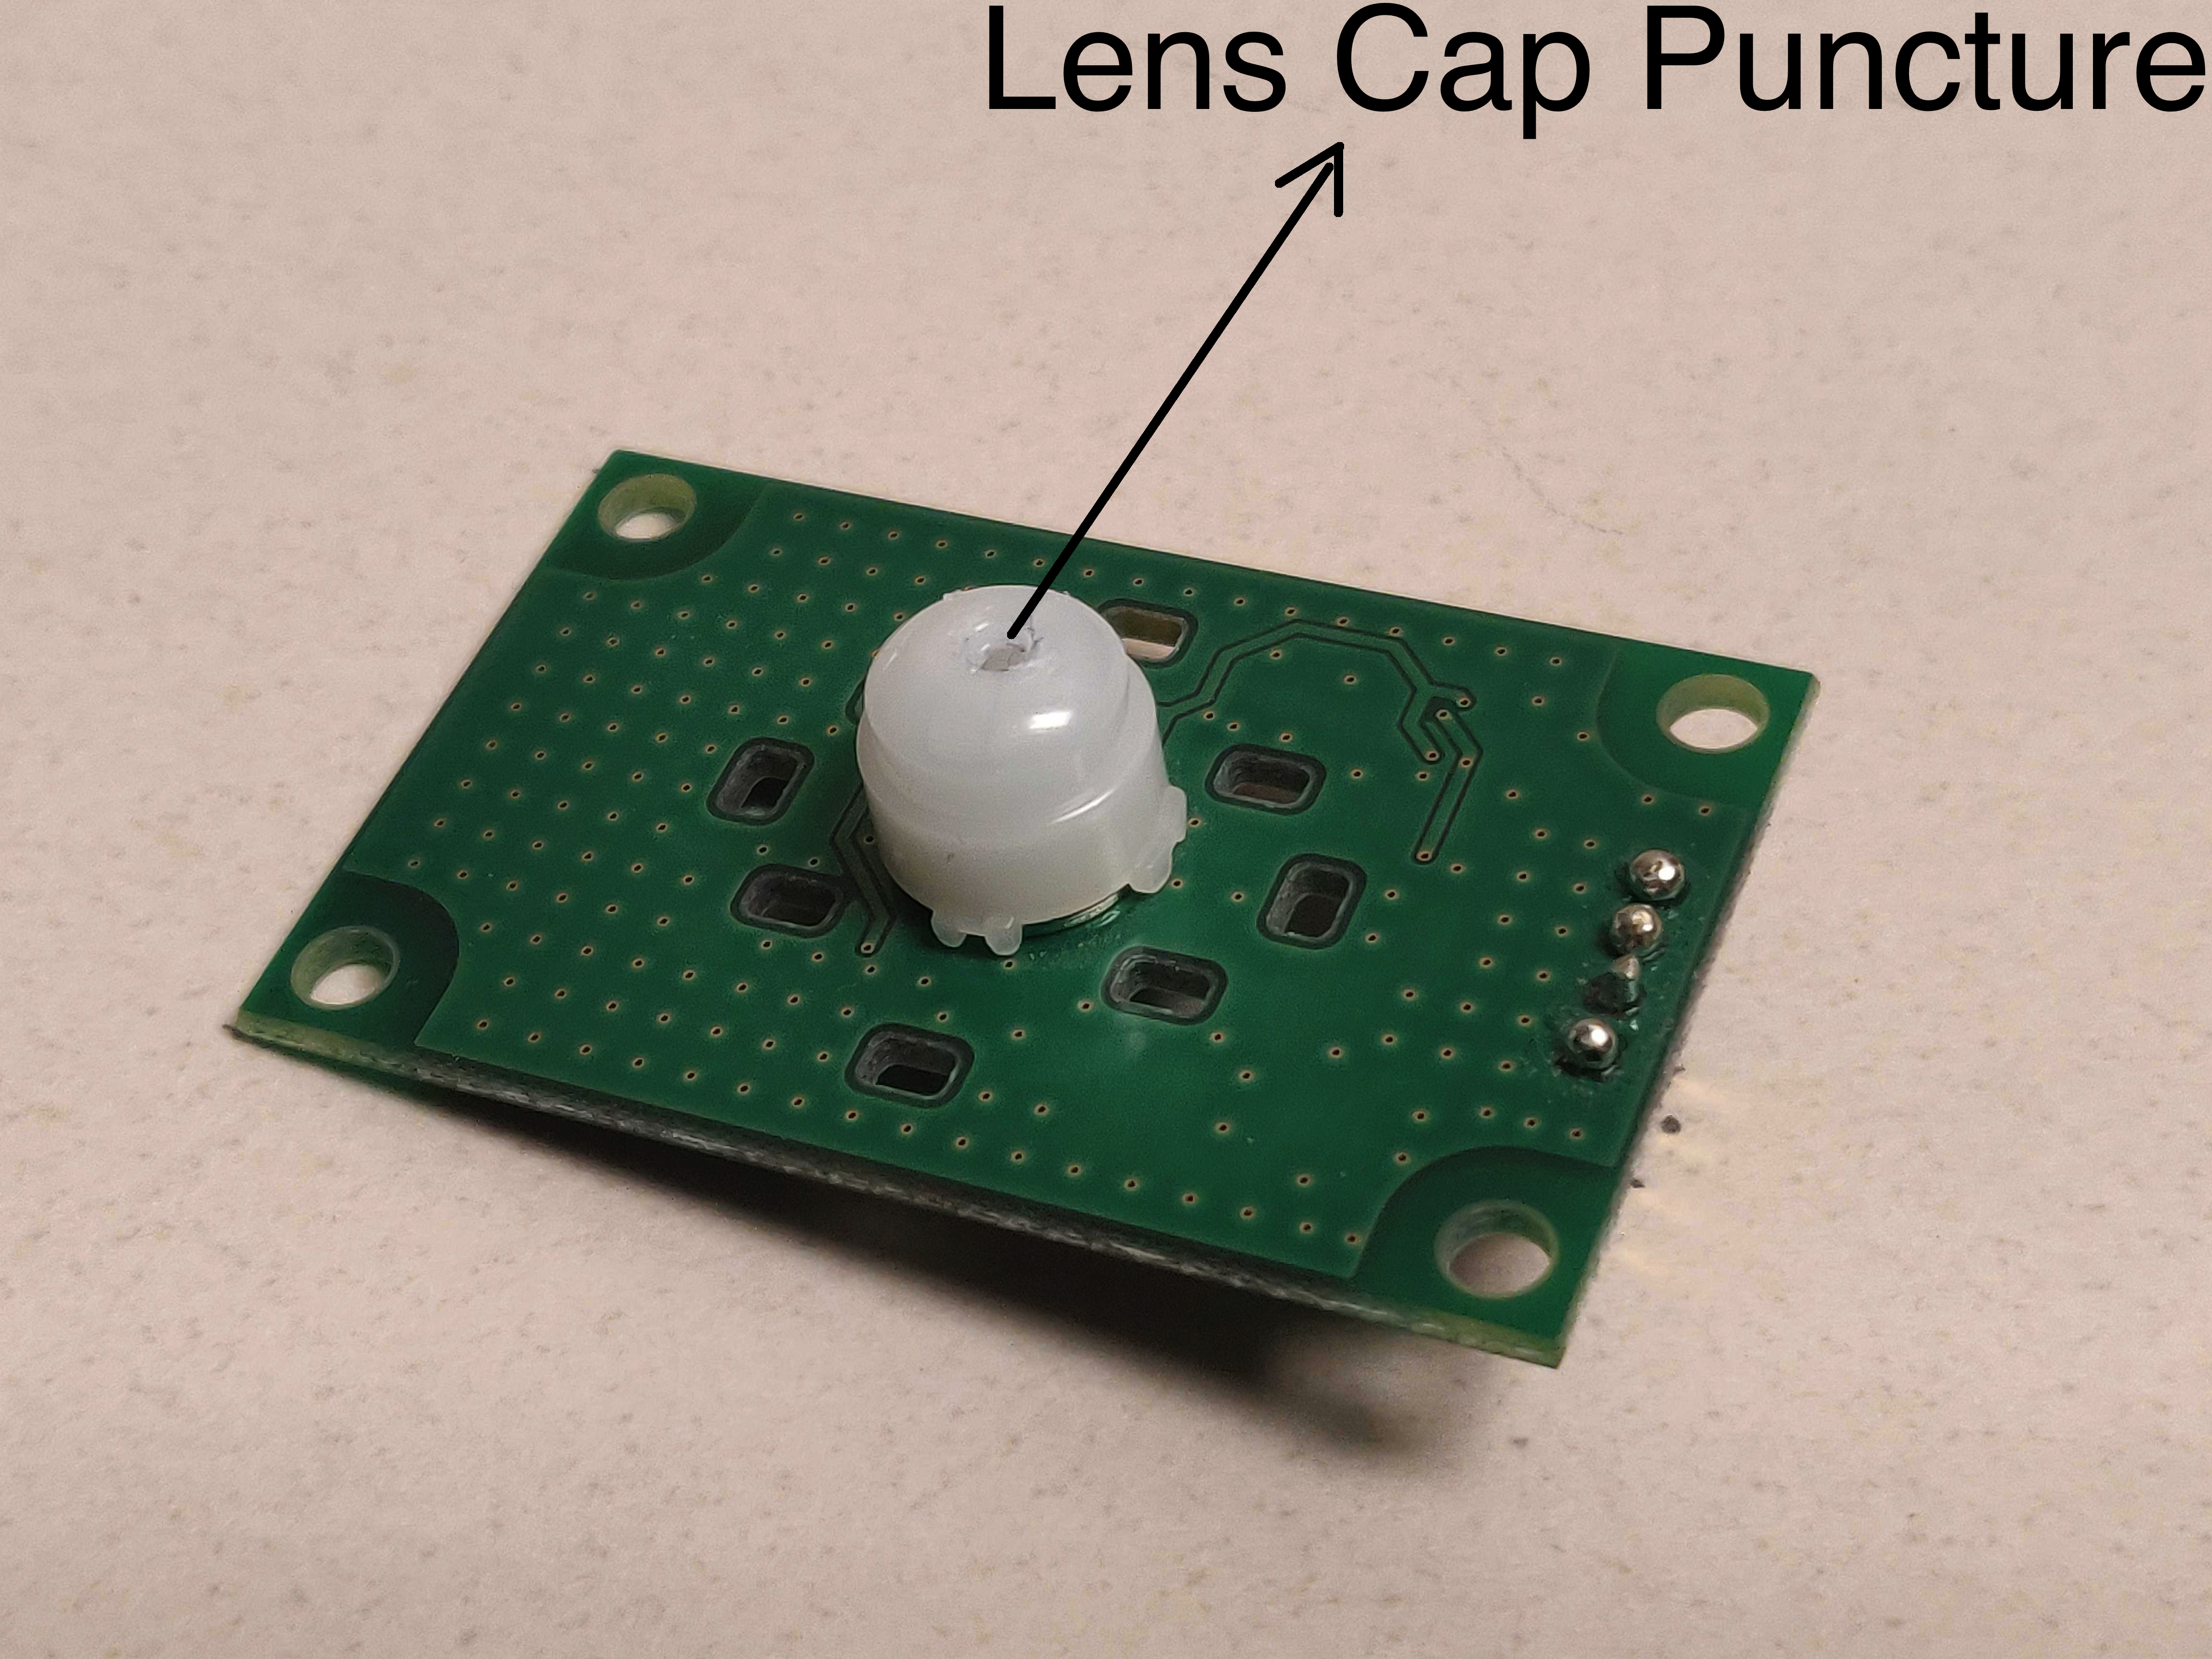
\includegraphics[width=\textwidth]{figures/platform/failure_photographs/ClassII-LensCapPunctured_new-2-annotated.png}
		\caption{Lens Cap Punctured}
		\label{fig:failure_photo4}
	\end{subfigure}
	\hspace{0.1ex}
	\begin{subfigure}[t]{0.24\textwidth}
		\centering
		\includegraphics[width=\textwidth]{figures/platform/failure_photographs/ClassIII-LensCapCovered-annotated-jpg.jpg}
		\caption{\footnotesize Lens Cap Covered}
		\label{fig:failure_photo5}
	\end{subfigure}
	\hspace{0.1ex}%
	\begin{subfigure}[t]{0.24\textwidth}
		\centering
		\includegraphics[width=\textwidth]{figures/platform/failure_photographs/ClassIV-OpticalFilterDamage-annotated-jpg.jpg}
		\caption{\footnotesize Optical Filter Damaged}
		\label{fig:failure_photo6}
	\end{subfigure}	
	\hspace{0.1ex}
	\begin{subfigure}[t]{0.24\textwidth}
		\centering
		\includegraphics[width=\textwidth]{figures/platform/failure_photographs/ClassV-ElectronicsFault-annotated-jpg.jpg}
		\caption{Electronic Fault}
		\label{fig:failure_photo7}
	\end{subfigure}	
	%\vspace{-10pt}
	\caption{\footnotesize{Some sensors} used in our study. Note that the failures are not always visually perceivable as the sensors are typically inaccessible.}
	\label{fig:pir_sensor_failure_photographs}
	%\vspace{-5pt}
\end{figure}

%%%%%%%%%%%%%%%%
% END OF FAILURE PHOTOGRAPHS
%%%%%%%%%%%%%%%%



%A PIR sensor can fail in multiple ways. Irrespective of the nature of failures, all failures lead to a compromised operation of the sensor resulting in data that is incorrect and lacking fidelity. 
Fundamentally, failures in a PIR sensor could occur either on the lens, the pyroelectric element or the electronics. We \textit{analyze and categorize practical, common and most frequent} failures as gathered in discussions with IoT engineers and technicians who install and maintain PIR sensor deployments. 
% We talked to technicians at our university building in the US as well as at our office building in India.
% Consequently, uncommon failures such as those due to cosmic rays and alpha-particles are outside the scope of this discussion. 
% Nevertheless, if the designer needs to account for esoteric failures, our framework provides a guideline for analysis.
%We next describe these common failures in each subsystem and study them in detail. 
We developed a new taxonomy for such failures, as summarized in {\bfseries Table~\ref{tab:pir_faults}} and visualized in {\bfseries Fig.~\ref{fig:pir_sensor_failure_photographs}}. 
% Note that failures are not necessarily binary in nature \ie there can be partial or temporary failures (degradation).

%\begin{table}%[b]
\begin{wraptable}{R}{0.65\textwidth}%[ht]\small
%\renewcommand{\arraystretch}{1.1}
%\vspace{-\baselineskip}
	\centering
	\footnotesize
    \caption{{\bfseries Taxonomy of Failures} in a PIR Sensor}
    \begin{tabular}{p{2.25cm} p{6cm}}
    \hline %\\
    \textsc{\bfseries Failure} & \textsc{\bfseries Definition \& Impact}\\
    \hline\hline
    \rowcolor{gray!20} \multicolumn{2}{l}{\bfseries Lens Subsystem}\\
    Lens dislodged \newline (Class I) & Lens cap suffers partial or complete dislocation \eg physical impact with a foreign object, degradation of bonding,~\etc \\
    Lens deformed \newline (Class II) & Lens cap suffers physical damage in-place \eg deformation, puncture,~\etc \\
    Lens covered \newline (Class III) & Lens cap gets physically obstructed by foreign particles \eg dust, paper or tape \\
    \hline
    \rowcolor{gray!20} \multicolumn{2}{l}{\bfseries Pyroelectric Subsystem} \\
    Optical filter \newline damage (Class IV) & Damaged by environmental factors~\eg oil condensation\\
    \hline
    \rowcolor{gray!20} \multicolumn{2}{l}{\bfseries Electronic Subsystem} \\
    Electronic faults \newline (Class V) & Hardware failures~\eg short circuits, floating outputs~\etc \\
    % Thermal Faults & Pyroelectric element can degrade or age and can give imperfect output\\
    \hline
    \end{tabular}
    \label{tab:pir_faults}
    %\vspace{-15pt}
    %\vspace{-\baselineskip}
\end{wraptable}
%\end{table}

\subsubsection{\textbf{Failures in the lens subsystem}} The lens is geometrically constructed to precisely focus the thermal rays onto the pyroelectric element. As a result, failures affecting the optical integrity of the lens can result in loss of precision for focusing the thermal rays. We observe three types of failures here, termed Class I--III failures.

\noindent \underline{Lens dislocation (Class I):} %Generally, the lens is either stuck onto the sensor board with an adhesive material or is constructed with hooks that latch onto the the sensor board (refer Fig. \ref{fig:pir_sensor_overview}). Thus, as a result of this, in deployment, 
As the lens is stuck on the sensor board with an adhesive or machined to fit over the pyroelectric element, it could get dislodged from its place or completely fall off the sensor board due to factors such as thermal expansion or physical impact. 
% We name these Class I failures.
%The result is loss of focus of thermal radiation on the pyroelectric element. 

\noindent \underline{Lens deformation (Class II):} As the lens is made of flexible, 0.4mm thick high density plastic~\cite{fresnel}, it is susceptible to deformation by physical damage. This can alter the curvature or puncture the lens. %We term such failures as Class II failures. 
%
As in Class I, the consequence of failure is imperfect capture and focusing of the thermal radiation incident on the PIR sensor.
%

\noindent \underline{Lens hindrance (Class III):} Dust particles (\eg factory floors, building construction) or common objects such as paper and plastic tape can absorb the thermal radiation resulting in reduced to no radiation falling on the pyroelectric element. The deposition of particulate matter also causes dispersion.
%These are termed Class III failures.% We refer to these as Class III failures.

In summary, Classes I--III failures affect the core functionality of the lens, and results in the imperfect capture and focus of thermal radiation.
%results in the imperfect capture and focus of thermal radiation thus affecting the core functionality of the lens.
% resulting in change in the ability of the lens to focus the narrow beam. 

\subsubsection{\textbf{Failures in the pyroelectric subsystem}: Optical Filter Damage (Class IV):} %The pyroelectric subsystem is another critical point of failure in a PIR sensor.  
The optical filter and pyroelectric elements are prone to degradation with exposure to high temperature and humidity. As the optical filter is carefully calibrated to trigger in the region of human motion, it is susceptible to damage due to environmental factors such as heat sources (\eg room heaters, air-conditioners) and humidity (\eg oil condensation) as it affects the perceived temperature of the object. We name these as Class IV failures.

\subsubsection{\textbf{Failures in the Electronics}} On-board electronics consisting of filter, amplifier and comparator circuitry are prone to failures such as shorted or floating pins that we refer to as Class V failures. We only consider simple, electronic failures -- such as open, short circuits and floating inputs. Vendor-based IC testing procedures and board design process advancements have made electronic failures such as regulator, bus failures and PCB malfunctions infrequent in practice.
%, and degradation due to elements such as temperature and humidity. 

%\noindent \textbf{Note:} In this study, we
%\st{do not consider hardware electronic failures such as PCB malfunctions and} 
%only consider simple electronics failures -- vendor-based IC testing procedures during board design process advancements have made electronics failures such as regulator failures, bus failures and PCB malfunctions infrequent.% one part per billion~\cite{}. 

%Instead, our focus is squarely on practical failures, and damage that can occur from the environment during deployment. We gathered these in discussion with PIR sensor manufacturers and smart building deployment technicians at our LEED-certified building. Lastly, we do not consider ageing of the PIR sensor separately as a fault. It is subsumed in the other failure scenarios.

\noindent \textbf{Summary:} Failures in PIR sensors can occur in either the lens subsystem, the pyroelectric subsystem or the on-board electronics, each of which manifest differently in the underlying physics.
%Each of these failures manifest differently in the underlying physics.% of sensing and thereby impact the sensor operation differently.


\subsection{Analyzing Severity of Failures -- A Quantitative Analysis}
\label{subsec:quantify}
A failure is said to impact the sensor performance if the failure results in either false detections ({\bfseries FD}) \ie false positives or missed obstacles ({\bfseries MO}) \ie false negatives in the sensor output (\cout), compared to a working sensor. As seen in {\bfseries Fig.~\ref{fig:pir_sensor_different_lens}}, \cout is HIGH (1) when no is obstacle detected and \cout goes HIGH (1) $\rightarrow$ LOW (0) when an obstacle is detected.

%To investigate the manner in which failure can affect the reliability of the PIR sensor, we investigate the output of the sensor \ie \cout. 

\noindent \underline{Controlled Failure Study:} To understand the impact on sensor performance, in our lab, we take 2 PIR sensors, one which is without the fault (\working) and one with the fault (\tampered). The 2 sensors are placed in as close a proximity to one another as possible such that -- \ca distance between the sensors are closer than the size of obstacle, \cb the obstacle is moved in a plane such that it comes into the detection region of both the PIR sensors simultaneously. This implies that when the obstacle (we used our palm in this case) is moved across the detection region of both PIR sensors, it grazed both at the same time, triggering the same responses from both the sensors.

We then calculate the absolute difference ($\delta_N$) between the \cout values of the tampered sensor~\viz  \couttampered and the reference working sensor~\viz \coutworking by summing over all observations (Refer Eqn.~\ref{eqn:1}). Intuitively, a relatively low $\delta_N$ would imply that the tampered sensor is still in acceptable condition \ie the failure is not having much impact on the operation of the sensor. On the other hand, a high value of difference implies that the failure is much serious. To ease computation, we can also compute $\delta_N$ by dividing the time series into equal size chunks called \textit{windows} (W) and computing the difference between average \cout values of \tampered and \working in that window.

\begin{table}%[b]
	\small
	\centering
	\caption{\textbf{Misclassifications} analysis for different failures. The numbers indicate the deviation (as defined in Eqn.~\ref{eqn:1} between $C_{out}$ values) of a faulty sensor from that of a working sensor. Higher number indicates increased degree of failure.}
	%\begin{tabular}{lcccc}
	\begin{tabular}{lllll}
		%\begin{tabular}{p{2cm}p{2cm}p{2cm}p{2cm}p{2cm}}
		\hline
		\bfseries \textsc{Failure} & \bfseries \textsc{Lens Dislodged} & \bfseries \textsc{Lens Covered} & \bfseries \textsc{Heat Damage} & \bfseries \textsc{Humidity Damage}\\
		\hline \hline
		\rowcolor{gray!20} $\delta_N$$^1$ & 35 & 48 & 29 & 48 \\
		$\delta_N$$^2$ & 69 & 94  & 53 & 87 \\
		\hline 
	\end{tabular}
	\label{tbl:fault_degree}
	%\vskip1pt
	\quad \raggedright
	$^1$ 6 hour run, $^2$ 12 hour run
\end{table} 

\textbf{Table~\ref{tbl:fault_degree}} summarizes $\delta_N$ for a few types of failures as observed over 6-hour and 12-hour runs deployed in the elevator of our building. The numbers in the column represent deviation or misclassifications ($\delta_N$)~\ie the number of false detections (both false positives and false negatives) by the faulty sensor calculated using {\bfseries Eqn.~\ref{eqn:1}}.
%In long deployments, 
We used a window size, $W$ = 1024 samples, which comes to a window of time duration slightly over 51 seconds at a sampling rate of 20 Hz.
In our case, the lens covered failure (8 failures per hour) is more pernicious than lens having fallen off (6 failures per hour).
% Equation working
%\begin{equation}
%    {\tikzmarknode{d}{\highlight{red}{$\delta_N$}}} = \underset{W}{\sum} \left|C_{\text{out,tampered}} - C_{\text{out, working}}\right|,
%    \label{eqn:1}
%    \begin{tikzpicture}[overlay,remember picture,>=stealth,nodes={align=left,inner ysep=1pt},<-]
	%        % For "d", i.e. delta
	%        \path (d.north) ++ (0,0.6em) node[anchor=south west,color=red!67] (scalep){\textbf{misclassifications}};
	%        \draw [color=red!57](d.north) |- ([xshift=-0.3ex,color=red]scalep.south east);
	%    \end{tikzpicture}
%\end{equation}

\begin{equation}
	{\tikzmarknode{d}{\highlight{blue}{$\delta_N$}}} = \underset{windows}{\sum} 
	\left| {\tikzmarknode{t}{\highlight{red}{$C_{\text{out,tampered}}$}}} - {\tikzmarknode{w}{\highlight{green}{$C_{\text{out, working}}$}}}\right|,
	\label{eqn:1}
	\begin{tikzpicture}[overlay,remember picture,>=stealth,nodes={align=left,inner ysep=1pt},<-]
		% For "d", i.e. delta
		\path (d.south) ++ (0,-0.6em) node[anchor=north east,color=blue!67] (scalep){\textbf{misclassifications}};
		\draw [color=blue!57](d.south) |- ([xshift=0.3ex,color=red]scalep.south west);
	\end{tikzpicture}
	\begin{tikzpicture}[overlay,remember picture,>=stealth,nodes={align=left,inner ysep=1pt},<-]
		% For "t", i.e. tampered
		\path (t.north) ++ (0,0.6em) node[anchor=south east,color=red!67] (scalep){\textbf{tampered}};
		\draw [color=red!57](t.north) |- ([xshift=-12ex,color=red]scalep.south east);
	\end{tikzpicture}
	\begin{tikzpicture}[overlay,remember picture,>=stealth,nodes={align=left,inner ysep=1pt},<-]
		% For "w", i.e. working
		\path (w.north) ++ (0,0.6em) node[anchor=south west,color=teal] (scalep){\textbf{working}};
		\draw [color=teal!57](w.north) |- ([xshift=-0.3ex,color=green]scalep.south east);
	\end{tikzpicture}
\end{equation}\\
%The degree of reliability required can be tuned according to the application. 
%\ashish{need a good terminology for false positive and false negatives.}

%\textbf{Granularity of Misclassifications} %A tunable parameter that arises while quantifying the impact of failure is the number of samples over which the misclassification is measured. The two extremes are -- \ca comparing sample by sample between the sensor values, and \cb capturing the entire measurement duration and comparing the (average) \cout values. More generally, To ease computation, we can also compute $\delta_N$ by dividing the time series into equal size chunks called \textit{windows} (W) and computing the difference between average \cout values of \tampered and \working. In long deployments, we used a window size, $W$ = 1024 samples, which comes to a window of time duration 40 seconds.

%In Table~\ref{tbl:fault_degree} we see that lens covered fault gives around 8 incorrect readings per hour compared to pyroelectric window broken scenario. We observe that obstruction due to foreign substances either on the lens or on the pyroelectric window can lead to highly erroneous sensor data.

\noindent \textbf{Summary:} Quantifying the impact of a failure gives hints on how pernicious specific failures are \textit{once they have been detected}.%We \textit{do not use Eqn~\ref{eqn:1} as a way to detect failures}. Instead, it serves as a guideline to develop a taxonomy of failures.




\begin{figure}[b]
	\centering
	\begin{subfigure}[b]{0.3\textwidth}
		\centering
		\includegraphics[scale=0.6, height=1.3in]{figures/platform/controlled_setup-2.png}
		\caption{Controlled Setup}
		\label{fig:pir_sensor_controlled}
	\end{subfigure}%
	\begin{subfigure}[t]{0.3\textwidth}
		\centering
		\includegraphics[width=\textwidth]{figures/2-PIR-Fault/normal-classI/classI_compared-again.png}
		\caption{Class I Fault}
		\label{fig:pir_sensor_controlled_a}
	\end{subfigure}%
	\begin{subfigure}[t]{0.3\textwidth}
		\centering
		\includegraphics[width=\textwidth]{figures/2-PIR-Fault/normal-classII/classII_compared.png}
		\caption{Class II Fault}
		\label{fig:pir_sensor_controlled_b}
	\end{subfigure}\\%
	\begin{subfigure}[t]{0.3\textwidth}
		\centering
		\includegraphics[width=\textwidth]{figures/2-PIR-Fault/normal-classIII/classIII_compared.png}
		\caption{Class III Fault}
		\label{fig:pir_sensor_controlled_c}
	\end{subfigure}
	\begin{subfigure}[t]{0.3\textwidth}
		\centering
		\includegraphics[width=\textwidth]{figures/2-PIR-Fault/normal-classIV/classIV_summary.png}
		\caption{Class IV Fault}
		\label{fig:pir_sensor_controlled_d}
	\end{subfigure}%
	\begin{subfigure}[t]{0.3\textwidth}
		\centering
		\includegraphics[width=\textwidth]{figures/2-PIR-Fault/normal-classV/classV_summary.png}
		\caption{Class V Fault}
		\label{fig:pir_sensor_controlled_e}
	\end{subfigure}
	\caption{(\ref{fig:pir_sensor_controlled_a} - \ref{fig:pir_sensor_controlled_e}) \footnotesize{\aout waveforms for sensor faults of Classes I--V}. Note that in Class I -- III faults, despite the obstacle still being detected, \aout provides indication of underlying abnormalities in the sensor.
	%We observe increased variance in Class I faults, reduced amplitude in Class II faults, and further reduced values of \aout in case of Class III faults. Note that in Class I -- III faults, despite the obstacle still being detected, \aout provides indication of underlying abnormalities in the sensor.In the Class IV fault, the optical filter has been contaminated by oil deposits, as could happen in factories. In the Class V fault, \aout is shorted to the power supply.
	}
	\label{fig:pir_sensor_controlled_classI-V}
%\vspace{-17pt}
\end{figure}

%%%%%%%%%%
%%% CAN MOVE THIS TO APPENDIX
%%%%%%%%%%%%




%\section{Characterizing Failures}